\documentclass[11pt,oneside]{article}
\usepackage[margin=1in]{geometry}
\usepackage{amsmath}
\usepackage{graphicx}
\usepackage{booktabs}
\usepackage{float}
\usepackage{subcaption}
\usepackage[font=footnotesize,labelfont=bf]{caption}
\usepackage{setspace}
\usepackage[colorlinks=true,allcolors=blue]{hyperref}

%%%%%%%%% Path resolution (Overleaf: tables/, plots/; Local: ../output/) %%%%%%%%%
\graphicspath{{plots/}{../output/plots/}}
\makeatletter
\def\input@path{{tables/}{../output/tables/}}
\makeatother

\linespread{1.3}

\title{Chat Embedding Analysis\\
\large Technical Report --- Issue \#42}
\author{Caleb Eynon}
\date{March 2026}

\begin{document}
\maketitle

\tableofcontents
\newpage

%% ============================================================
\section{Methods}
%% ============================================================

\subsection{Embedding Models}

We embed chat messages using two OpenAI models:
\begin{itemize}
    \item \texttt{text-embedding-3-small} (1,536 dimensions)
    \item \texttt{text-embedding-3-large} (3,072 dimensions)
\end{itemize}

Embeddings are computed at two granularities:
\begin{enumerate}
    \item \textbf{Message level}: each chat message embedded individually (4,700 messages).
    \item \textbf{Player-round level}: all messages from one player in one round concatenated before embedding (2,298 texts).
\end{enumerate}

Chat messages are paired with the contribution they influenced (the next round's decision). Round 1 of each supergame has no associated chat.

\subsection{Direction Vectors}

For a binary label (positive/negative), we compute:
\begin{align}
    \mathbf{c}_+ &= \frac{1}{n_+} \sum_{i \in \text{positive}} \mathbf{e}_i \\
    \mathbf{c}_- &= \frac{1}{n_-} \sum_{i \in \text{negative}} \mathbf{e}_i \\
    \mathbf{d} &= \frac{\mathbf{c}_+ - \mathbf{c}_-}{\|\mathbf{c}_+ - \mathbf{c}_-\|}
\end{align}
Each embedding is then projected onto the direction: $s_i = \mathbf{e}_i \cdot \mathbf{d}$.

\subsection{Five Direction Axes}

\begin{table}[H]
\centering
\caption{Direction vector definitions}
\label{tab:directions}
\footnotesize
\begin{tabular}{llllr}
\toprule
Direction & Positive class & Label level & Source file & Positive $n$ \\
\midrule
Cooperative & \texttt{player\_state == cooperative} & Player & \texttt{player\_state\_classification.csv} & 3,800 \\
Promise & \texttt{classification == 1} & Message & \texttt{promise\_classifications.csv} & 2,195 \\
Homogeneity & contribution range $\leq 1$ ECU & Group-round & computed from contributions & 520 \\
Round liar & \texttt{lied\_this\_round\_20 == True} & Player-round & \texttt{behavior\_classifications.csv} & 94 \\
Cumulative liar & \texttt{is\_liar\_20 == True} & Player-round & \texttt{behavior\_classifications.csv} & 113 \\
\bottomrule
\end{tabular}
\end{table}

\subsection{Probe Phrase Validation}

For each direction, we embed predefined probe phrases and compute cosine similarity with $\mathbf{d}$:
\begin{equation}
    \text{sim}(\mathbf{p}, \mathbf{d}) = \frac{\mathbf{p} \cdot \mathbf{d}}{\|\mathbf{p}\|}
\end{equation}

\subsection{Logistic Regression}

5-fold stratified cross-validated logistic regression at the player-round level. Dependent variable: \texttt{high\_contribution} ($\geq 20$ out of 25 ECU). Four feature sets per direction:
\begin{enumerate}
    \item VADER only (4 sentiment features)
    \item Projection only (1-dimensional projection score)
    \item Full embedding (PCA reduced to 50 components)
    \item VADER + Projection
\end{enumerate}

\subsection{Panel Regression}

Fixed-effects panel regressions using \texttt{fixest::feols()} in R. Fixed effects: round + segment. Clustering: session $\times$ segment $\times$ group. Two dependent variables: group contribution (0--100) and others' contribution (0--75). Each projection type enters as a separate specification.

%% ============================================================
\section{Scripts}
%% ============================================================

\subsection{Embedding Pipeline}

\begin{tabular}{ll}
\toprule
Script & Purpose \\
\midrule
\texttt{compute\_embeddings.py} & Call OpenAI API, cache as Parquet \\
\texttt{merge\_panel\_data.py} & Integrate 20 projection columns into panel \\
\bottomrule
\end{tabular}

\subsection{Analysis Drivers}

\begin{tabular}{ll}
\toprule
Script & Direction \\
\midrule
\texttt{analyze\_embeddings.py} & Cooperative \\
\texttt{analyze\_promise\_embeddings.py} & Promise \\
\texttt{analyze\_homogeneity\_embeddings.py} & Homogeneity \\
\texttt{analyze\_round\_liar\_embeddings.py} & Round liar \\
\texttt{analyze\_cumulative\_liar\_embeddings.py} & Cumulative liar \\
\bottomrule
\end{tabular}

\medskip
Each driver: loads cached embeddings $\rightarrow$ computes centroids and direction vector $\rightarrow$ projects all messages $\rightarrow$ runs probe validation $\rightarrow$ saves projection CSV.

\subsection{Regression Scripts}

\begin{tabular}{ll}
\toprule
Script & Output table \\
\midrule
\texttt{embedding\_regression.py} & \texttt{embedding\_regression\_comparison.tex} \\
\texttt{promise\_embedding\_regression.py} & \texttt{promise\_embedding\_regression\_comparison.tex} \\
\texttt{homogeneity\_embedding\_regression.py} & \texttt{homogeneity\_embedding\_regression\_comparison.tex} \\
\texttt{round\_liar\_embedding\_regression.py} & \texttt{round\_liar\_embedding\_regression\_comparison.tex} \\
\texttt{cumulative\_liar\_embedding\_regression.py} & \texttt{cumulative\_liar\_embedding\_regression\_comparison.tex} \\
\texttt{group\_contribution\_embedding\_regression.R} & \texttt{group\_contribution\_embedding\_regression.tex} \\
 & \texttt{others\_contribution\_embedding\_regression.tex} \\
\bottomrule
\end{tabular}

\subsection{Visualization Scripts}

\begin{tabular}{ll}
\toprule
Script & Plots \\
\midrule
\texttt{embedding\_plots.py} & UMAP, t-SNE, projection distributions (cooperative) \\
\texttt{promise\_embedding\_plots.py} & UMAP, t-SNE, projection distributions (promise) \\
\bottomrule
\end{tabular}

%% ============================================================
\section{Outputs}
%% ============================================================

\subsection{Probe Phrase Validation}

\begin{table}[H]
\centering
\caption{Cooperative direction --- probe phrases (small model)}
\label{tab:probe_coop}
\footnotesize
\begin{tabular}{lr}
\toprule
Phrase & Cosine sim. \\
\midrule
``I'm going to free ride'' & $+0.04$ \\
``put in everything'' & $-0.02$ \\
``we should cooperate'' & $-0.08$ \\
``I don't trust them'' & $-0.12$ \\
``let's all contribute 25'' & $-0.13$ \\
``I'll put in zero'' & $-0.19$ \\
\bottomrule
\end{tabular}
\end{table}

\begin{table}[H]
\centering
\caption{Promise direction --- probe phrases (small / large model)}
\label{tab:probe_promise}
\footnotesize
\begin{tabular}{lrr}
\toprule
Phrase & Small & Large \\
\midrule
``I promise to put in 25'' & $+0.47$ & $+0.40$ \\
``let's all commit to the max'' & $+0.25$ & $+0.29$ \\
``we all agreed to cooperate'' & $+0.22$ & $+0.25$ \\
``trust me I'll do my part'' & $+0.21$ & $+0.22$ \\
``I swear I'll put in everything'' & $+0.19$ & $+0.19$ \\
``I'll contribute the full amount'' & $+0.19$ & $+0.26$ \\
``I said I would contribute'' & $+0.15$ & $+0.18$ \\
``I'll do whatever I want'' & $+0.15$ & $+0.17$ \\
``no guarantees from me'' & $+0.13$ & $+0.11$ \\
``I might change my mind'' & $+0.11$ & $+0.10$ \\
``I never said I'd do anything'' & $+0.08$ & $+0.14$ \\
``I'm not making any promises'' & $+0.08$ & $+0.11$ \\
\bottomrule
\end{tabular}
\end{table}

\begin{table}[H]
\centering
\caption{Homogeneity direction --- probe phrases (small / large model)}
\label{tab:probe_homog}
\footnotesize
\begin{tabular}{lrr}
\toprule
Phrase & Small & Large \\
\midrule
``we're all on the same page'' & $-0.01$ & $-0.01$ \\
``I'll match whatever you do'' & $-0.01$ & $-0.06$ \\
``I'm going my own way'' & $-0.02$ & $+0.01$ \\
``I'll do what the group does'' & $-0.03$ & $-0.06$ \\
``let's coordinate our contributions'' & $-0.12$ & $-0.15$ \\
``I don't care what others do'' & $-0.12$ & $-0.09$ \\
``everyone do 25'' & $-0.14$ & $-0.11$ \\
``some of us are free riding'' & $-0.16$ & $-0.07$ \\
``I'm putting in zero'' & $-0.24$ & $-0.24$ \\
``we should all contribute equally'' & $-0.25$ & $-0.27$ \\
``let's all put in the same amount'' & $-0.27$ & $-0.29$ \\
\bottomrule
\end{tabular}
\end{table}

\begin{table}[H]
\centering
\caption{Round-liar direction --- probe phrases (small / large model)}
\label{tab:probe_rliar}
\footnotesize
\begin{tabular}{lrr}
\toprule
Phrase & Small & Large \\
\midrule
``I changed my mind'' & $+0.19$ & $+0.16$ \\
``I promise to put in 25'' & $+0.15$ & $+0.11$ \\
``I'll put in everything'' & $+0.14$ & $+0.12$ \\
``I said I'd cooperate but I didn't'' & $+0.12$ & $+0.12$ \\
``I always do what I say'' & $+0.11$ & $+0.12$ \\
``trust me'' & $+0.09$ & $+0.10$ \\
``I kept my word'' & $+0.04$ & $+0.03$ \\
``someone is not being honest'' & $+0.01$ & $+0.01$ \\
``I lied about my contribution'' & $-0.01$ & $-0.01$ \\
``I never break a promise'' & $-0.01$ & $+0.01$ \\
``they lied to us'' & $-0.08$ & $-0.03$ \\
\bottomrule
\end{tabular}
\end{table}

\begin{table}[H]
\centering
\caption{Cumulative-liar direction --- probe phrases (small / large model)}
\label{tab:probe_cliar}
\footnotesize
\begin{tabular}{lrr}
\toprule
Phrase & Small & Large \\
\midrule
``I promise to put in 25'' & $+0.26$ & $+0.25$ \\
``I lied about my contribution'' & $+0.21$ & $+0.20$ \\
``I changed my mind'' & $+0.18$ & $+0.12$ \\
``I said I would but I didn't'' & $+0.17$ & $+0.15$ \\
``I kept my word'' & $+0.10$ & $+0.04$ \\
``I'm going to free ride'' & $+0.06$ & $+0.02$ \\
``trust me'' & $+0.06$ & $+0.04$ \\
``I'll contribute everything'' & $+0.01$ & $+0.02$ \\
``we should cooperate'' & $-0.02$ & $-0.01$ \\
``let's all be honest'' & $-0.03$ & $-0.01$ \\
\bottomrule
\end{tabular}
\end{table}

\subsection{Logistic Regression Tables}

\begin{table}[H]
\caption{Cooperative direction: 5-fold CV logistic regression}
\label{tab:reg_coop}
\begingroup
\centering
\begin{tabular}{lccccc}
   \tabularnewline \midrule \midrule
   Model & ACCURACY & AUC & PRECISION & RECALL & F1 \\
   \midrule
   VADER only & 0.7811 & 0.6198 & 0.7857 & 0.9884 & 0.8754 \\
   Projection only & 0.7990 & 0.7576 & 0.8130 & 0.9633 & 0.8818 \\
   Full embedding (PCA 50) & 0.8081 & 0.7540 & 0.8357 & 0.9383 & 0.8837 \\
   VADER + Projection & 0.7976 & 0.7648 & 0.8128 & 0.9614 & 0.8808 \\
   \midrule \midrule
   \multicolumn{6}{l}{\emph{5-fold stratified cross-validation}}\\
\end{tabular}
\par\endgroup

\end{table}

\begin{table}[H]
\caption{Promise direction: 5-fold CV logistic regression}
\label{tab:reg_promise}
\begingroup
\centering
\begin{tabular}{lccccc}
   \tabularnewline \midrule \midrule
   Model & ACCURACY & AUC & PRECISION & RECALL & F1 \\
   \midrule
   VADER only & 0.6282 & 0.6730 & 0.6122 & 0.4125 & 0.4911 \\
   Promise projection only & 0.8096 & 0.8968 & 0.7875 & 0.7732 & 0.7799 \\
   Full embedding (PCA 50) & 0.8142 & 0.8853 & 0.7850 & 0.7904 & 0.7870 \\
   VADER + Promise proj. & 0.8051 & 0.8999 & 0.7829 & 0.7663 & 0.7736 \\
   \midrule \midrule
   \multicolumn{6}{l}{\emph{5-fold stratified cross-validation}}\\
\end{tabular}
\par\endgroup

\end{table}

\begin{table}[H]
\caption{Homogeneity direction: 5-fold CV logistic regression}
\label{tab:reg_homog}
\input{homogeneity_embedding_regression_comparison}
\end{table}

\begin{table}[H]
\caption{Round-liar direction: 5-fold CV logistic regression}
\label{tab:reg_rliar}
\begingroup
\centering
\begin{tabular}{lccccc}
   \tabularnewline \midrule \midrule
   Model & ACCURACY & AUC & PRECISION & RECALL & F1 \\
   \midrule
   VADER only & 0.8903 & 0.5766 & 0.8903 & 1.0000 & 0.9420 \\
   Round-liar proj. only & 0.8908 & 0.6140 & 0.8907 & 1.0000 & 0.9422 \\
   Full embedding (PCA 50) & 0.8916 & 0.7129 & 0.8970 & 0.9922 & 0.9422 \\
   VADER + Round-liar proj. & 0.8903 & 0.6710 & 0.8924 & 0.9971 & 0.9418 \\
   \midrule \midrule
   \multicolumn{6}{l}{\emph{5-fold stratified CV, player-round level}}\\
\end{tabular}
\par\endgroup

\end{table}

\begin{table}[H]
\caption{Cumulative-liar direction: 5-fold CV logistic regression}
\label{tab:reg_cliar}
\input{cumulative_liar_embedding_regression_comparison}
\end{table}

\subsection{Panel Regression Tables}

\begin{table}[H]
\caption{Group contribution on embedding projections (fixest, FE: round + segment)}
\label{tab:panel_group}

\begingroup
\centering
\begin{tabular}{lccccc}
   \tabularnewline \midrule \midrule
   Dependent Variable: & \multicolumn{5}{c}{group\_contribution}\\
                   & Cooperative    & Promise         & Homogeneity    & Round-liar      & Cumulative-liar \\   
   Model:          & (1)            & (2)             & (3)            & (4)             & (5)\\  
   \midrule
   \emph{Variables}\\
   Cooperative     & 50.36$^{***}$  &                 &                &                 &   \\   
                   & (6.315)        &                 &                &                 &   \\   
   Word Count      & 0.2332$^{***}$ & -0.2178$^{***}$ & 0.2092$^{***}$ & -0.2840$^{***}$ & 0.0833\\   
                   & (0.0786)       & (0.0760)        & (0.0778)       & (0.0808)        & (0.0778)\\   
   Promise         &                & -7.158          &                &                 &   \\   
                   &                & (5.408)         &                &                 &   \\   
   Homogeneity     &                &                 & 49.41$^{***}$  &                 &   \\   
                   &                &                 & (6.451)        &                 &   \\   
   Round-liar      &                &                 &                & -41.37$^{***}$  &   \\   
                   &                &                 &                & (9.018)         &   \\   
   Cumulative-liar &                &                 &                &                 & -41.55$^{***}$\\   
                   &                &                 &                &                 & (6.765)\\   
   \midrule
   \emph{Fixed-effects}\\
   round           & Yes            & Yes             & Yes            & Yes             & Yes\\  
   segment         & Yes            & Yes             & Yes            & Yes             & Yes\\  
   \midrule
   \emph{Fit statistics}\\
   Observations    & 2,298          & 2,298           & 2,298          & 2,298           & 2,298\\  
   R$^2$           & 0.15240        & 0.08925         & 0.14974        & 0.10792         & 0.12005\\  
   \midrule \midrule
   \multicolumn{6}{l}{\emph{Clustered (cluster\_id) standard-errors in parentheses}}\\
   \multicolumn{6}{l}{\emph{Signif. Codes: ***: 0.01, **: 0.05, *: 0.1}}\\
\end{tabular}
\par\endgroup



\end{table}

\begin{table}[H]
\caption{Others' contribution on embedding projections (fixest, FE: round + segment)}
\label{tab:panel_others}

\begingroup
\centering
\begin{tabular}{lccccc}
   \tabularnewline \midrule \midrule
   Dependent Variable: & \multicolumn{5}{c}{others\_contribution}\\
                   & Cooperative    & Promise         & Homogeneity   & Round-liar      & Cumulative-liar \\   
   Model:          & (1)            & (2)             & (3)           & (4)             & (5)\\  
   \midrule
   \emph{Variables}\\
   Cooperative     & 41.74$^{***}$  &                 &               &                 &   \\   
                   & (5.200)        &                 &               &                 &   \\   
   Word Count      & 0.1740$^{***}$ & -0.2017$^{***}$ & 0.1495$^{**}$ & -0.2430$^{***}$ & 0.0384\\   
                   & (0.0643)       & (0.0629)        & (0.0640)      & (0.0661)        & (0.0635)\\   
   Promise         &                & -8.028$^{*}$    &               &                 &   \\   
                   &                & (4.307)         &               &                 &   \\   
   Homogeneity     &                &                 & 40.40$^{***}$ &                 &   \\   
                   &                &                 & (5.282)       &                 &   \\   
   Round-liar      &                &                 &               & -27.77$^{***}$  &   \\   
                   &                &                 &               & (6.878)         &   \\   
   Cumulative-liar &                &                 &               &                 & -32.83$^{***}$\\   
                   &                &                 &               &                 & (5.305)\\   
   \midrule
   \emph{Fixed-effects}\\
   round           & Yes            & Yes             & Yes           & Yes             & Yes\\  
   segment         & Yes            & Yes             & Yes           & Yes             & Yes\\  
   \midrule
   \emph{Fit statistics}\\
   Observations    & 2,298          & 2,298           & 2,298         & 2,298           & 2,298\\  
   R$^2$           & 0.15349        & 0.08500         & 0.14873       & 0.09644         & 0.11436\\  
   \midrule \midrule
   \multicolumn{6}{l}{\emph{Clustered (cluster\_id) standard-errors in parentheses}}\\
   \multicolumn{6}{l}{\emph{Signif. Codes: ***: 0.01, **: 0.05, *: 0.1}}\\
\end{tabular}
\par\endgroup



\end{table}

\subsection{Summary Comparison}

\begin{table}[H]
\centering
\caption{Summary comparison of direction vectors}
\label{tab:comparison}
\footnotesize
\begin{tabular}{lccccc}
\toprule
& Cooperative & Promise & Homogeneity & Round Liar & Cum.\ Liar \\
\midrule
Label level & Player & Message & Group-round & Player-round & Player-round \\
Label source & player\_state & promise\_class. & contributions & behavior\_class. & behavior\_class. \\
Probe validation & Inverted & Correct & Inverted & Mixed & Partial \\
Positive class $n$ & 3,800 & 2,195 & 520 & 94 & 113 \\
Projection-only AUC & 0.76 & 0.90 & 0.67 & 0.61 & 0.63 \\
VADER-only AUC & 0.62 & 0.67 & 0.58 & 0.58 & 0.58 \\
\bottomrule
\end{tabular}
\end{table}

\subsection{Visualizations}

\begin{figure}[H]
\centering
\begin{subfigure}[b]{0.48\textwidth}
    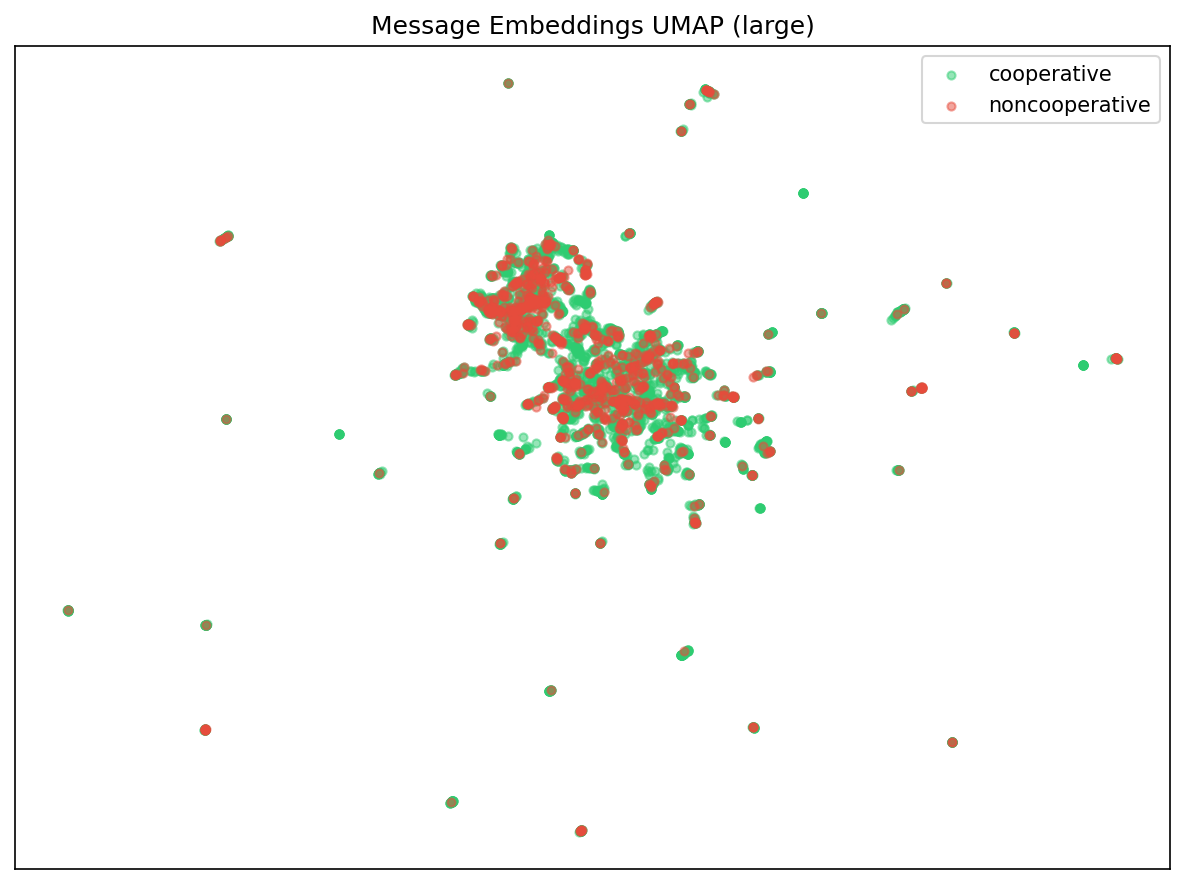
\includegraphics[width=\textwidth]{embedding_umap_large}
    \caption{UMAP --- cooperative}
\end{subfigure}
\hfill
\begin{subfigure}[b]{0.48\textwidth}
    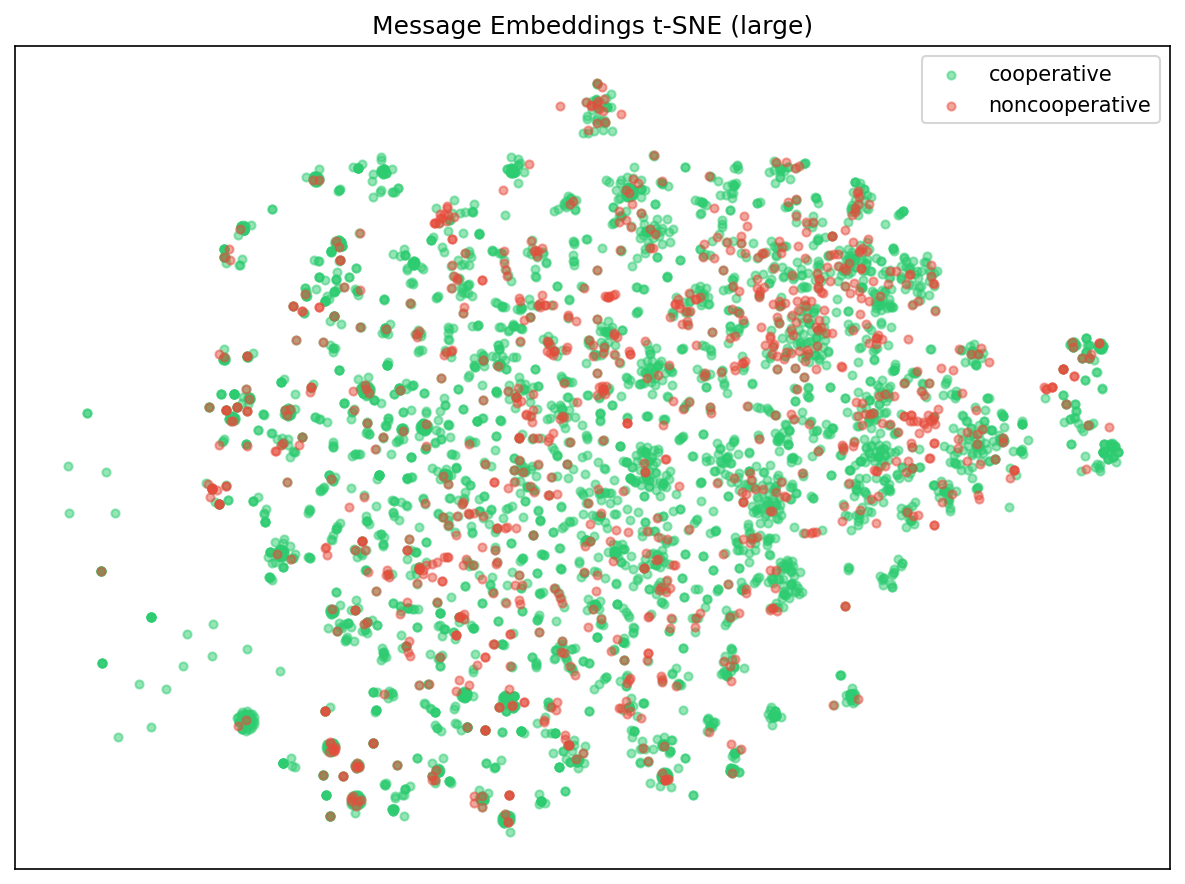
\includegraphics[width=\textwidth]{embedding_tsne_large}
    \caption{t-SNE --- cooperative}
\end{subfigure}
\caption{Message embeddings colored by cooperative state (large model).}
\label{fig:coop_dimreduce}
\end{figure}

\begin{figure}[H]
\centering
\begin{subfigure}[b]{0.48\textwidth}
    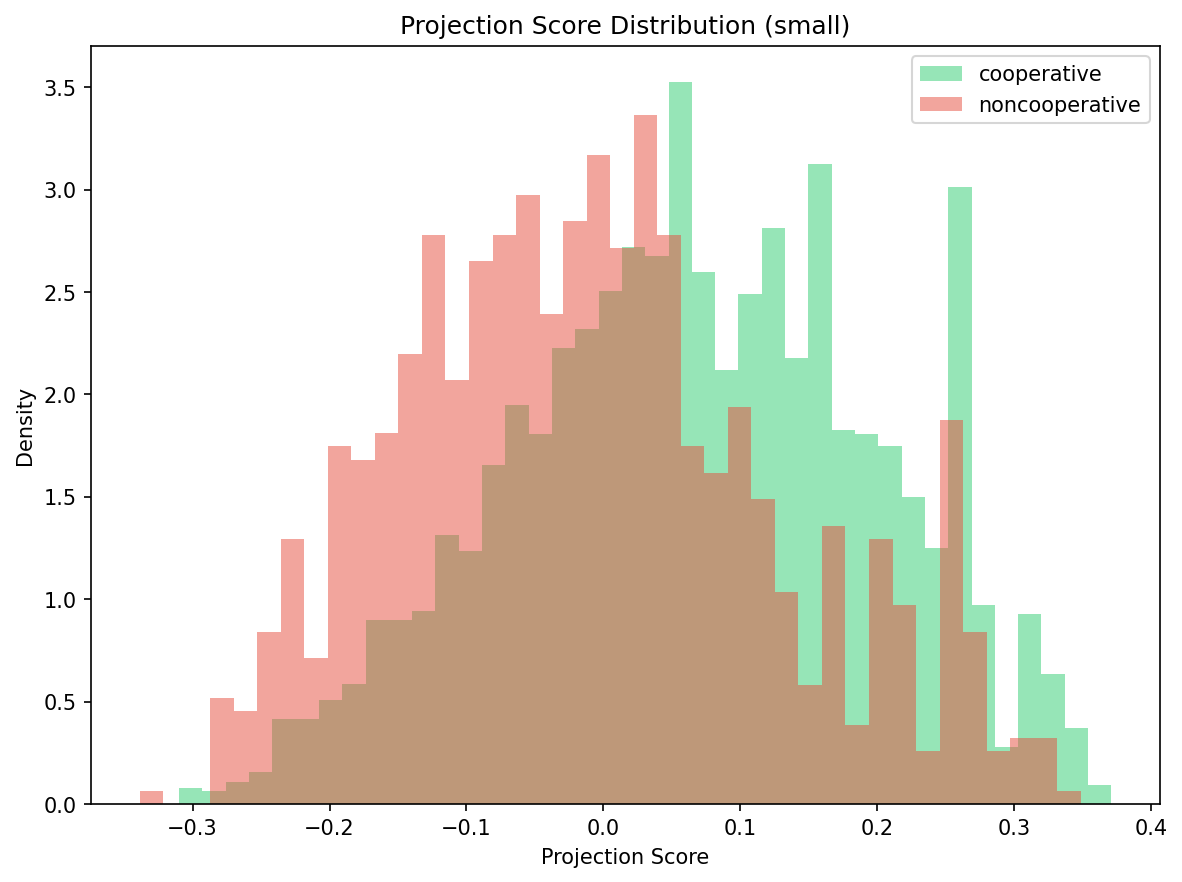
\includegraphics[width=\textwidth]{embedding_projection_dist_small}
    \caption{Small model}
\end{subfigure}
\hfill
\begin{subfigure}[b]{0.48\textwidth}
    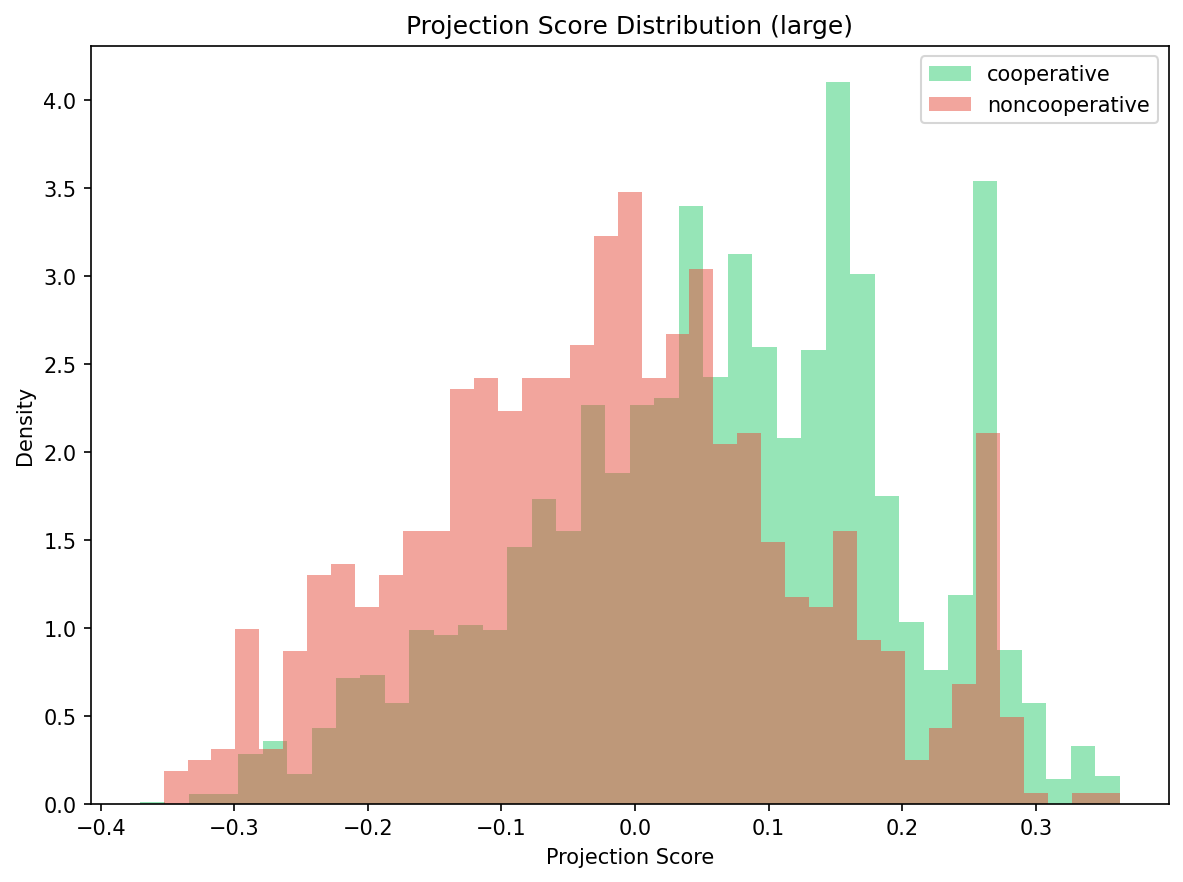
\includegraphics[width=\textwidth]{embedding_projection_dist_large}
    \caption{Large model}
\end{subfigure}
\caption{Cooperative direction projection score distributions by state.}
\label{fig:coop_projdist}
\end{figure}

\begin{figure}[H]
\centering
\begin{subfigure}[b]{0.48\textwidth}
    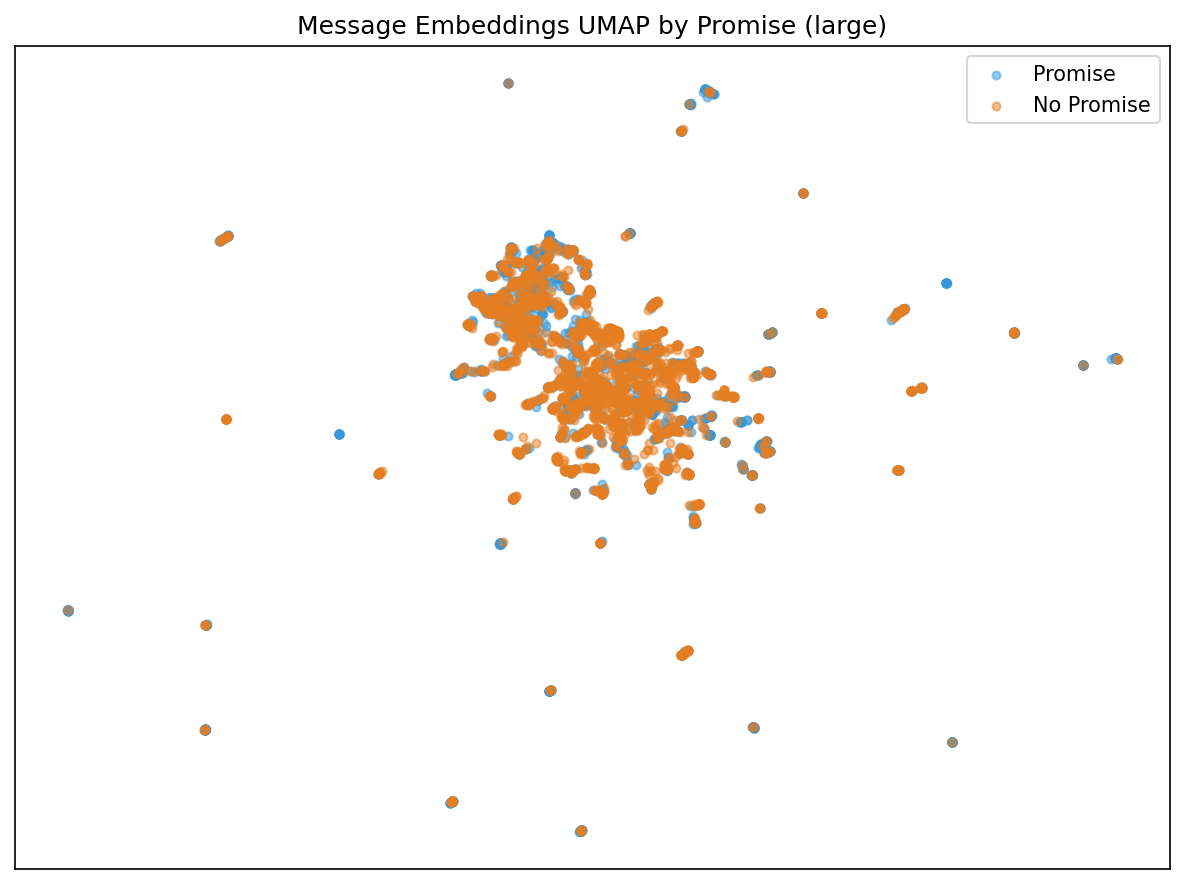
\includegraphics[width=\textwidth]{promise_umap_large}
    \caption{UMAP --- promise}
\end{subfigure}
\hfill
\begin{subfigure}[b]{0.48\textwidth}
    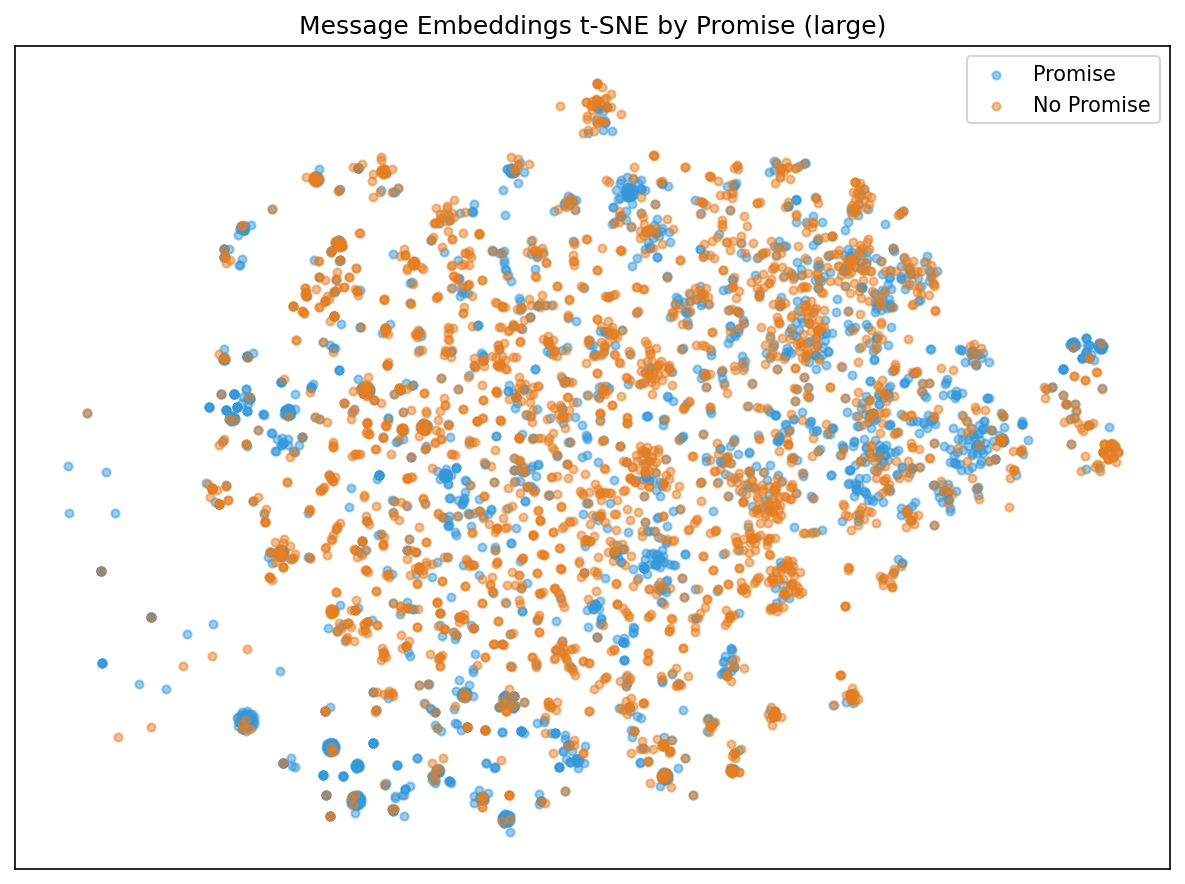
\includegraphics[width=\textwidth]{promise_tsne_large}
    \caption{t-SNE --- promise}
\end{subfigure}
\caption{Message embeddings colored by promise state (large model).}
\label{fig:promise_dimreduce}
\end{figure}

\begin{figure}[H]
\centering
\begin{subfigure}[b]{0.48\textwidth}
    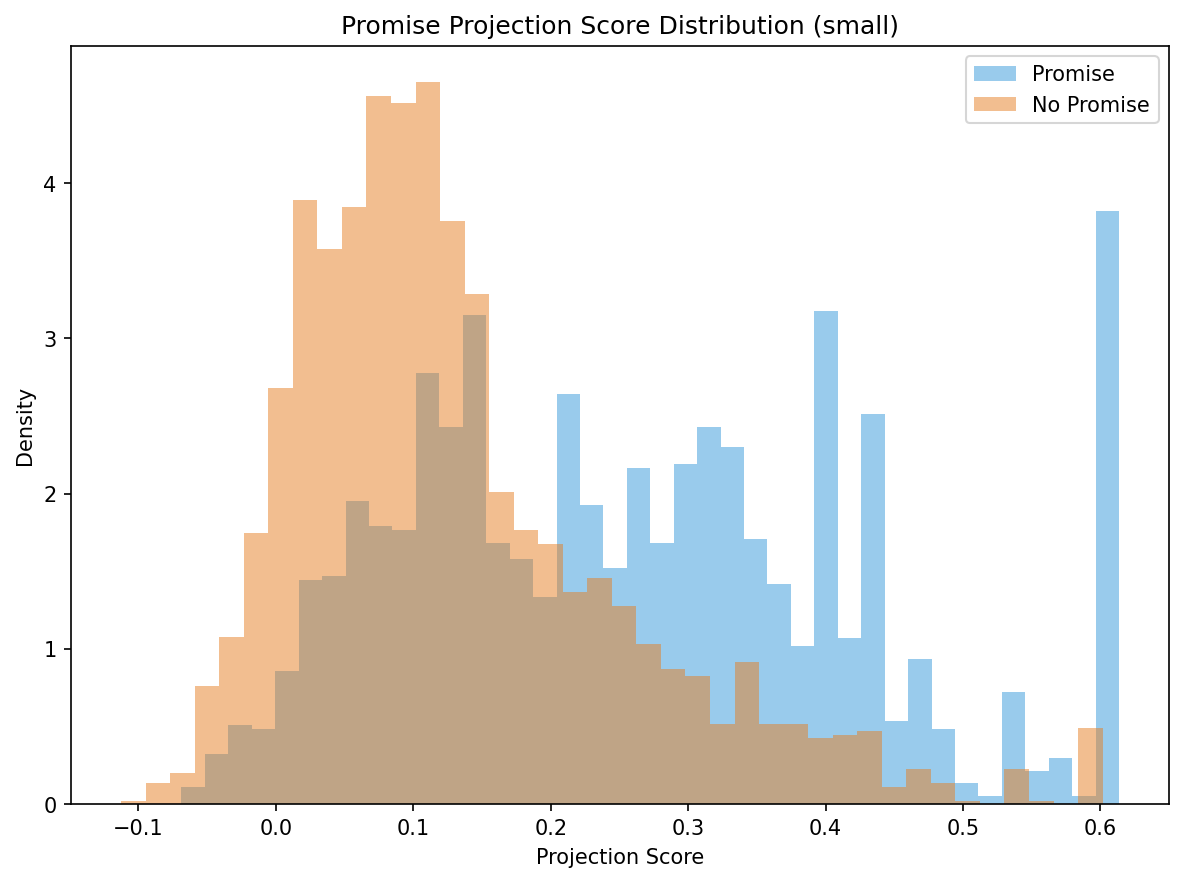
\includegraphics[width=\textwidth]{promise_projection_dist_small}
    \caption{Small model}
\end{subfigure}
\hfill
\begin{subfigure}[b]{0.48\textwidth}
    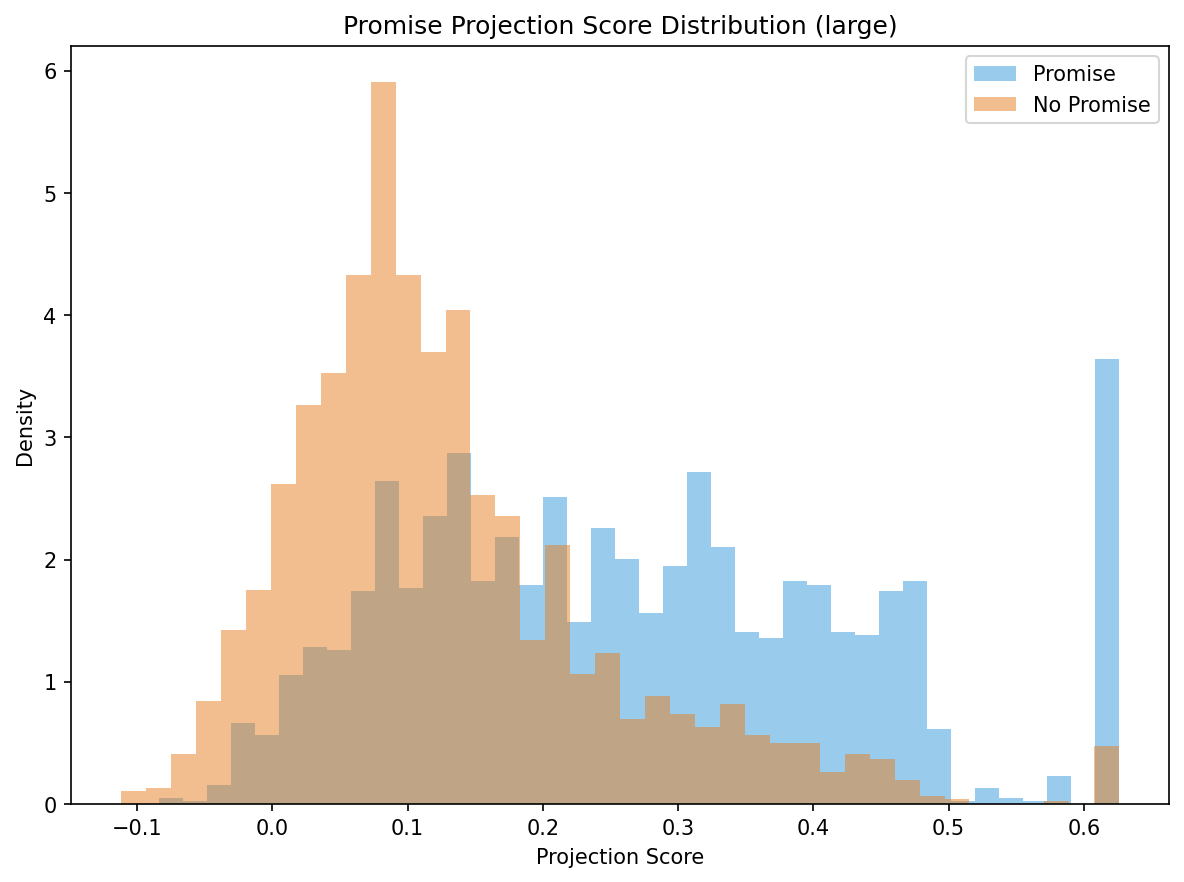
\includegraphics[width=\textwidth]{promise_projection_dist_large}
    \caption{Large model}
\end{subfigure}
\caption{Promise direction projection score distributions by state.}
\label{fig:promise_projdist}
\end{figure}

\begin{figure}[H]
\centering
\begin{subfigure}[b]{0.48\textwidth}
    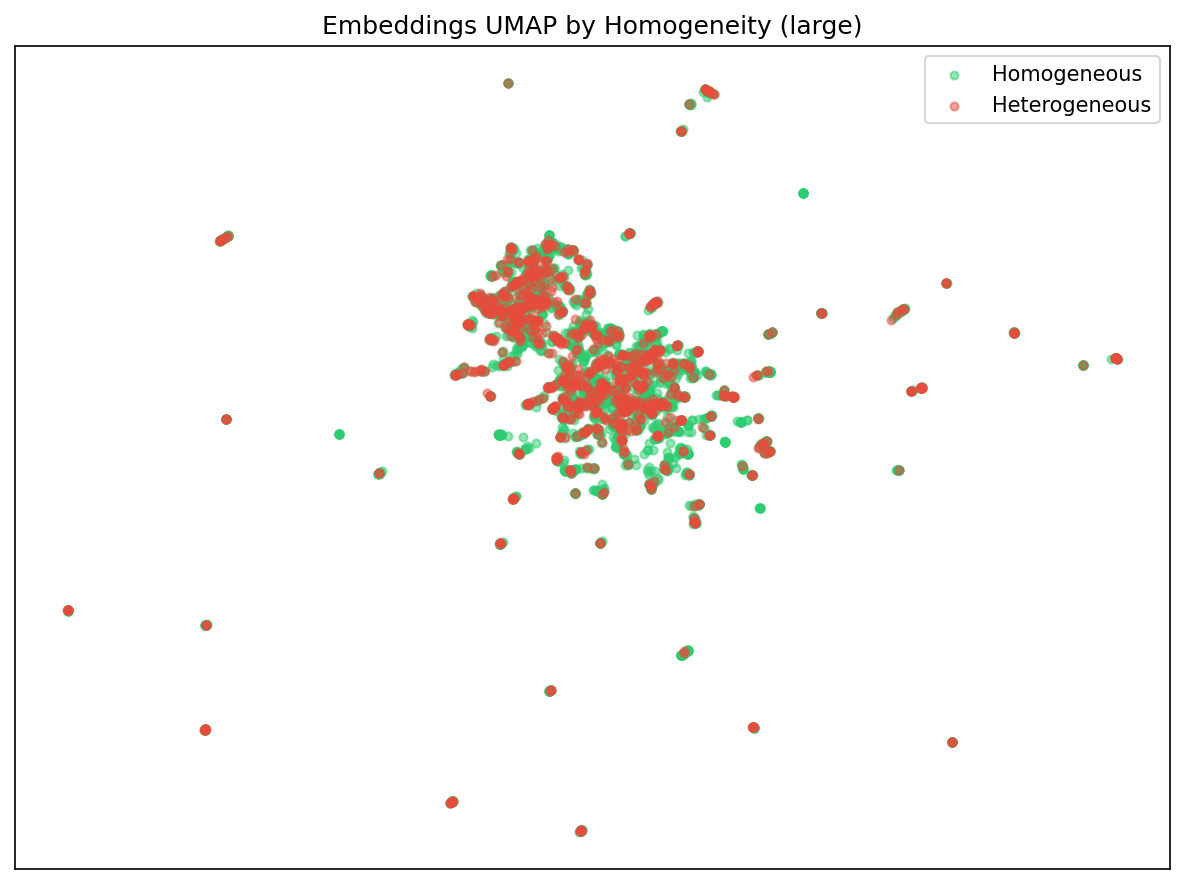
\includegraphics[width=\textwidth]{homogeneity_umap_large}
    \caption{UMAP --- homogeneity}
\end{subfigure}
\hfill
\begin{subfigure}[b]{0.48\textwidth}
    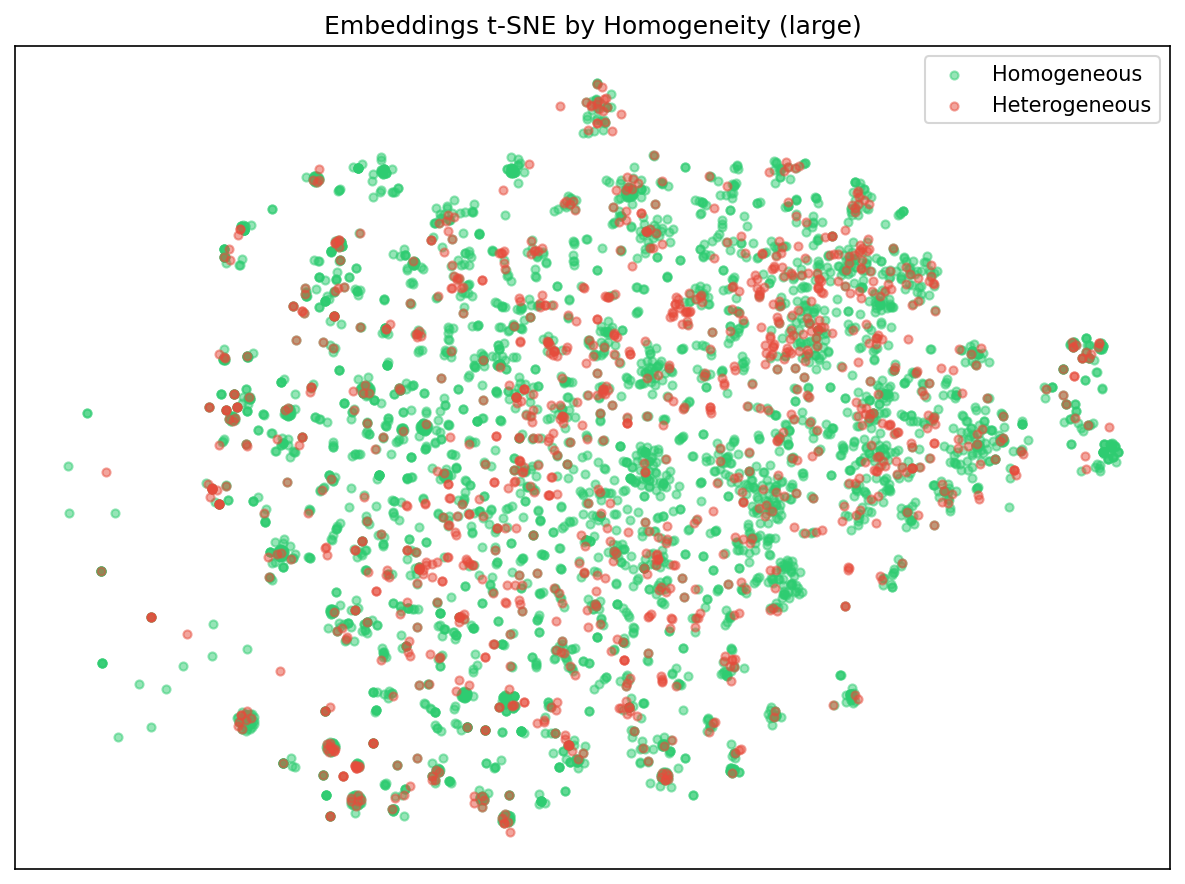
\includegraphics[width=\textwidth]{homogeneity_tsne_large}
    \caption{t-SNE --- homogeneity}
\end{subfigure}
\caption{Message embeddings colored by contribution homogeneity (large model).}
\label{fig:homog_dimreduce}
\end{figure}

\begin{figure}[H]
\centering
\begin{subfigure}[b]{0.48\textwidth}
    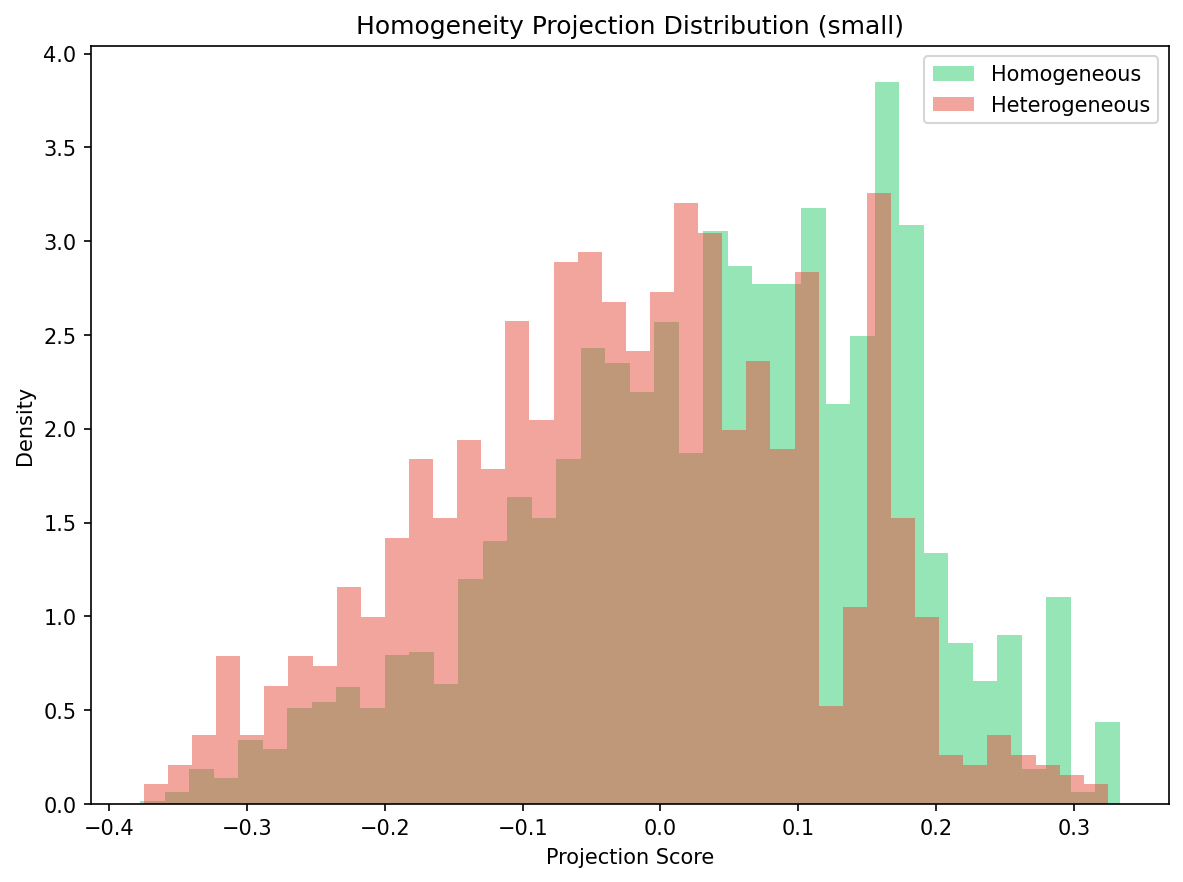
\includegraphics[width=\textwidth]{homogeneity_projection_dist_small}
    \caption{Small model}
\end{subfigure}
\hfill
\begin{subfigure}[b]{0.48\textwidth}
    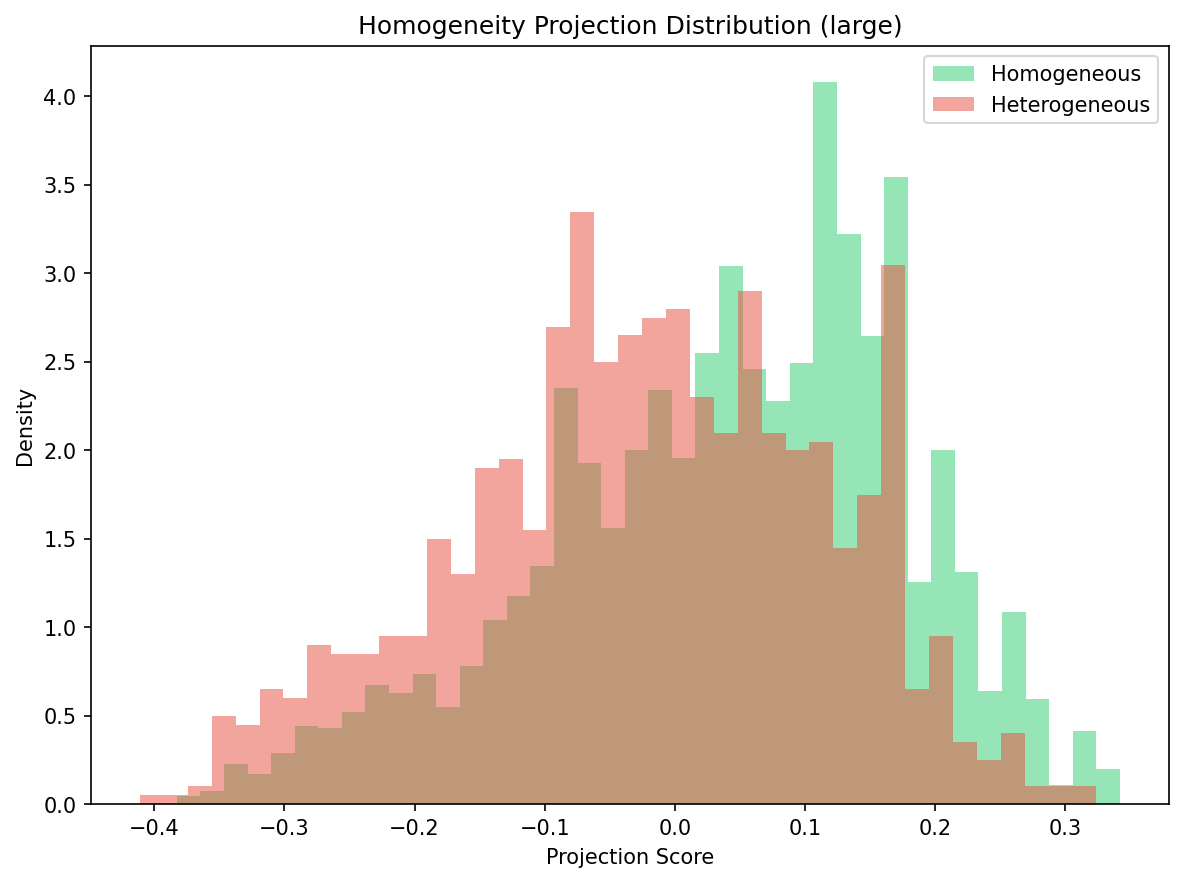
\includegraphics[width=\textwidth]{homogeneity_projection_dist_large}
    \caption{Large model}
\end{subfigure}
\caption{Homogeneity direction projection score distributions by state.}
\label{fig:homog_projdist}
\end{figure}

\begin{figure}[H]
\centering
\begin{subfigure}[b]{0.48\textwidth}
    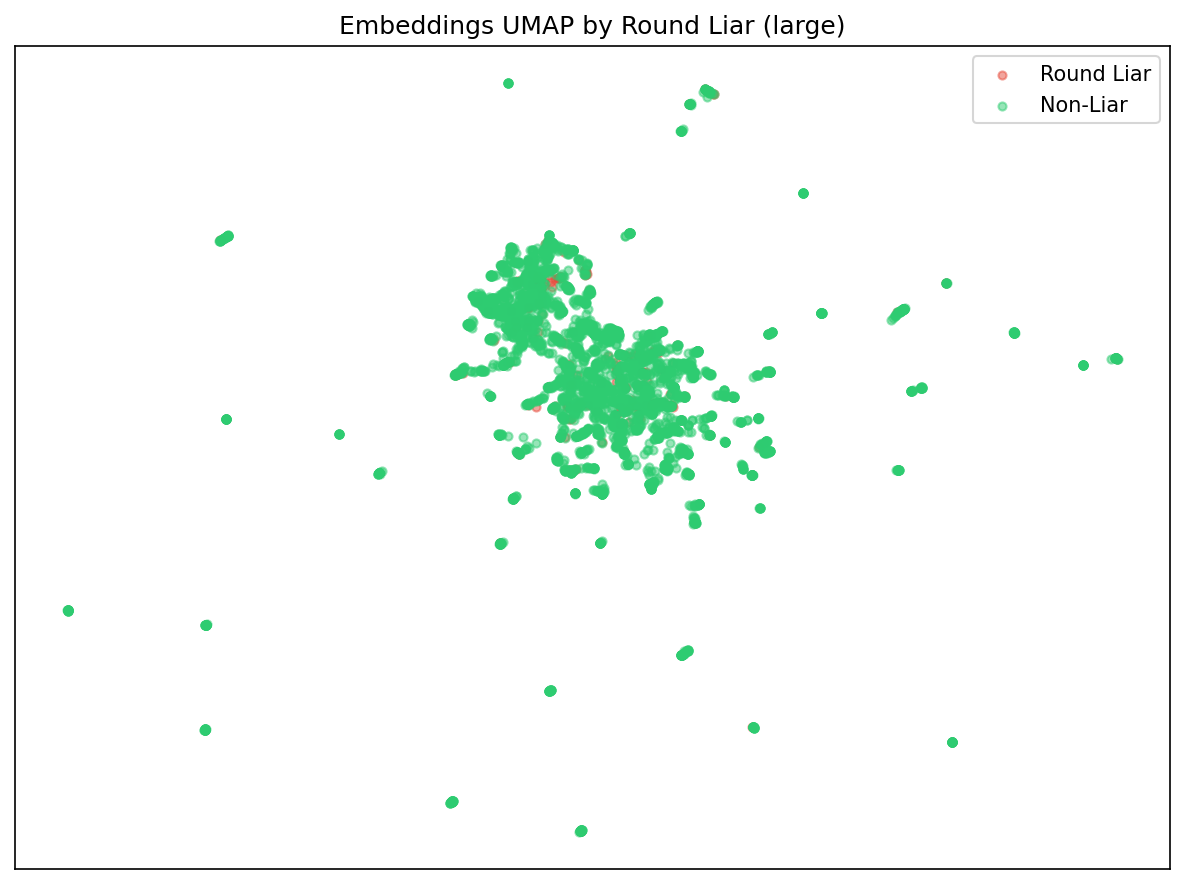
\includegraphics[width=\textwidth]{round_liar_umap_large}
    \caption{UMAP --- round liar}
\end{subfigure}
\hfill
\begin{subfigure}[b]{0.48\textwidth}
    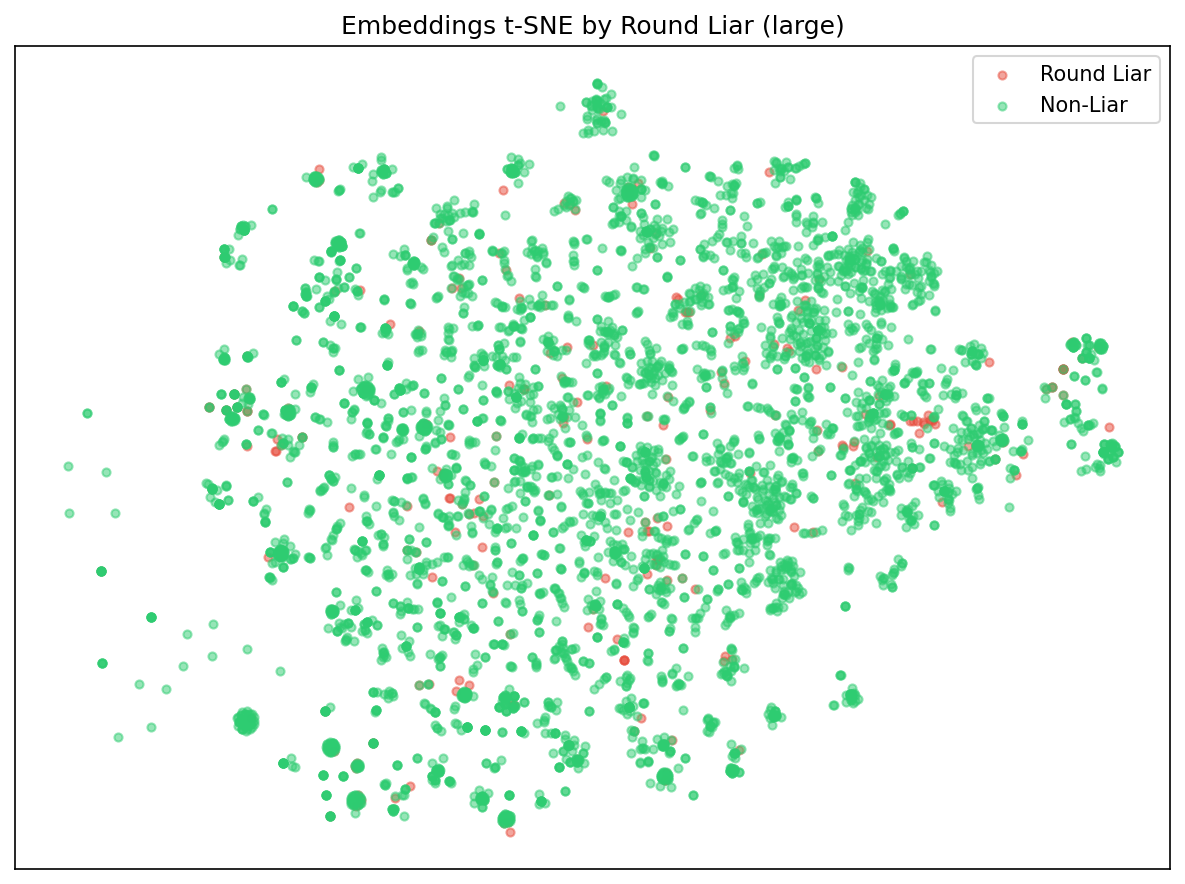
\includegraphics[width=\textwidth]{round_liar_tsne_large}
    \caption{t-SNE --- round liar}
\end{subfigure}
\caption{Message embeddings colored by round-liar status (large model).}
\label{fig:rliar_dimreduce}
\end{figure}

\begin{figure}[H]
\centering
\begin{subfigure}[b]{0.48\textwidth}
    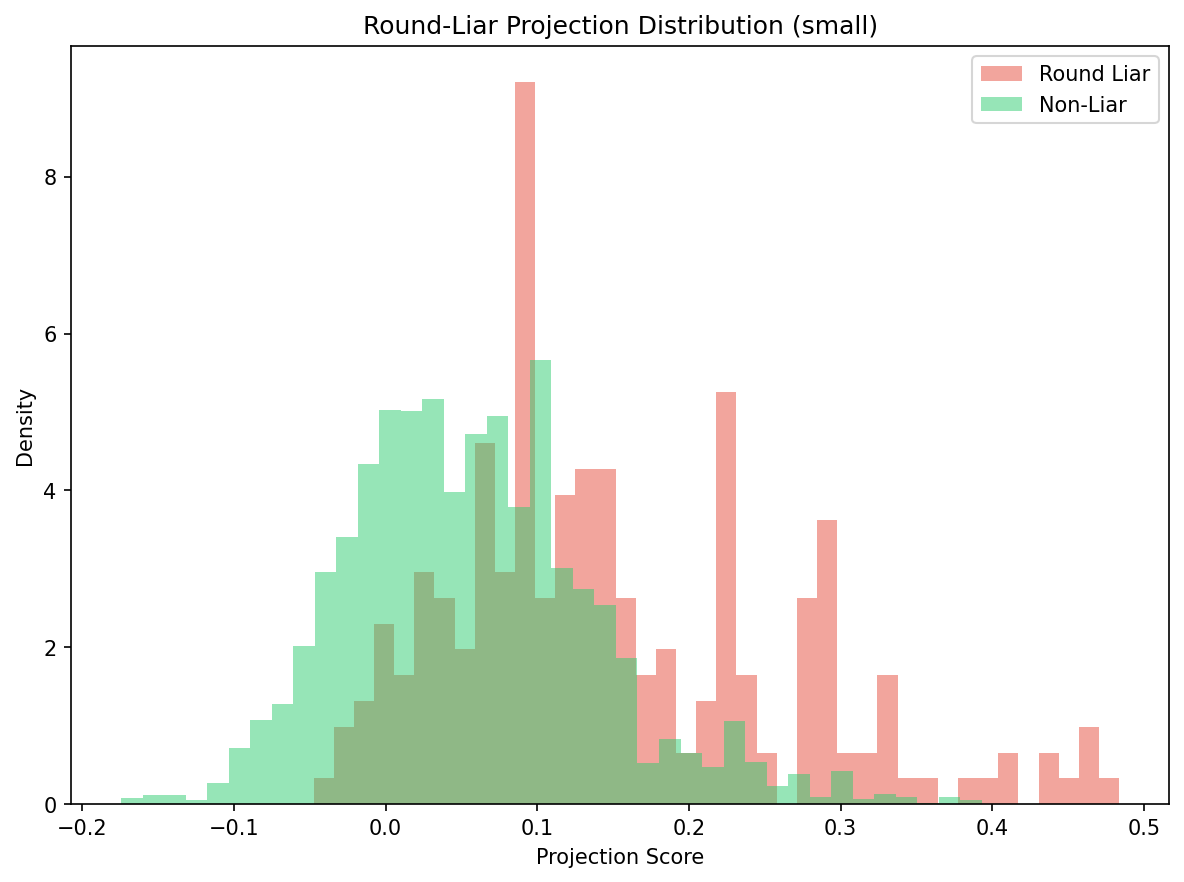
\includegraphics[width=\textwidth]{round_liar_projection_dist_small}
    \caption{Small model}
\end{subfigure}
\hfill
\begin{subfigure}[b]{0.48\textwidth}
    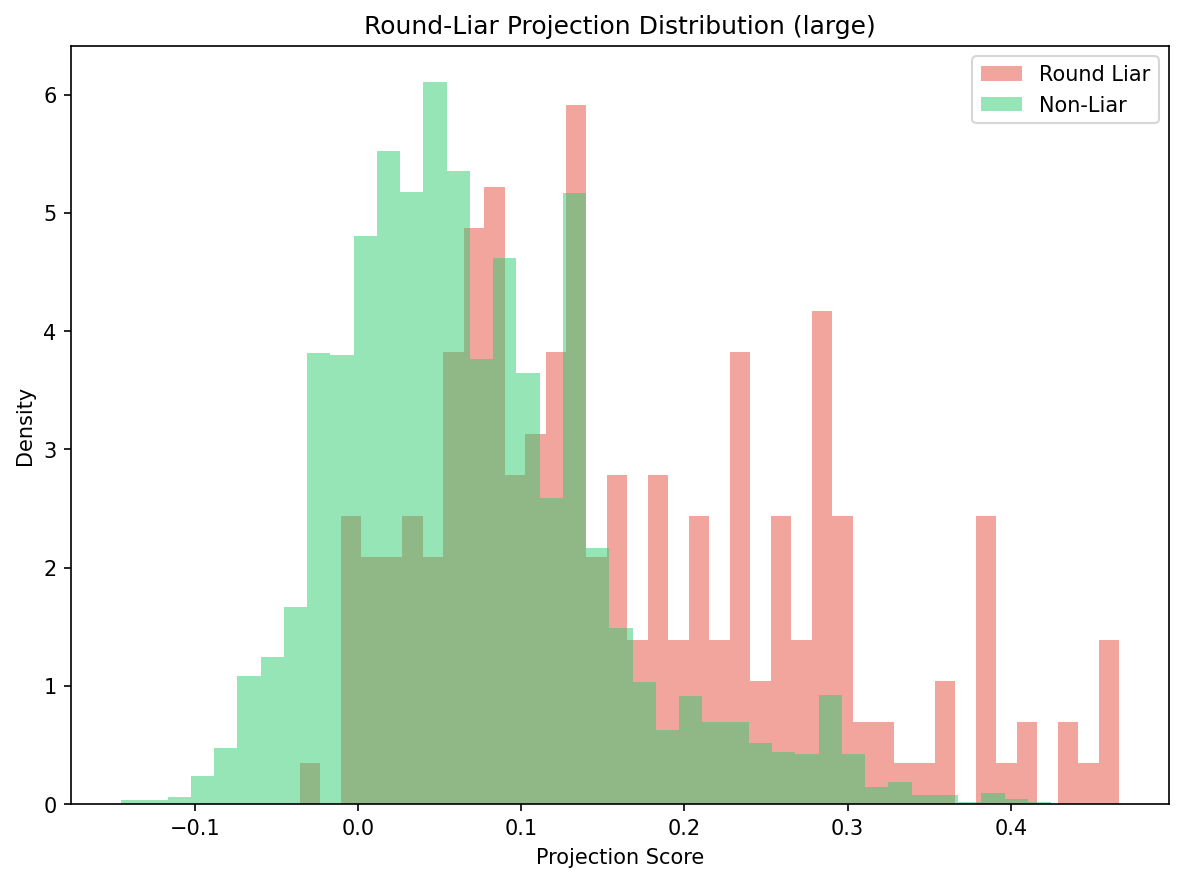
\includegraphics[width=\textwidth]{round_liar_projection_dist_large}
    \caption{Large model}
\end{subfigure}
\caption{Round-liar direction projection score distributions by state.}
\label{fig:rliar_projdist}
\end{figure}

\begin{figure}[H]
\centering
\begin{subfigure}[b]{0.48\textwidth}
    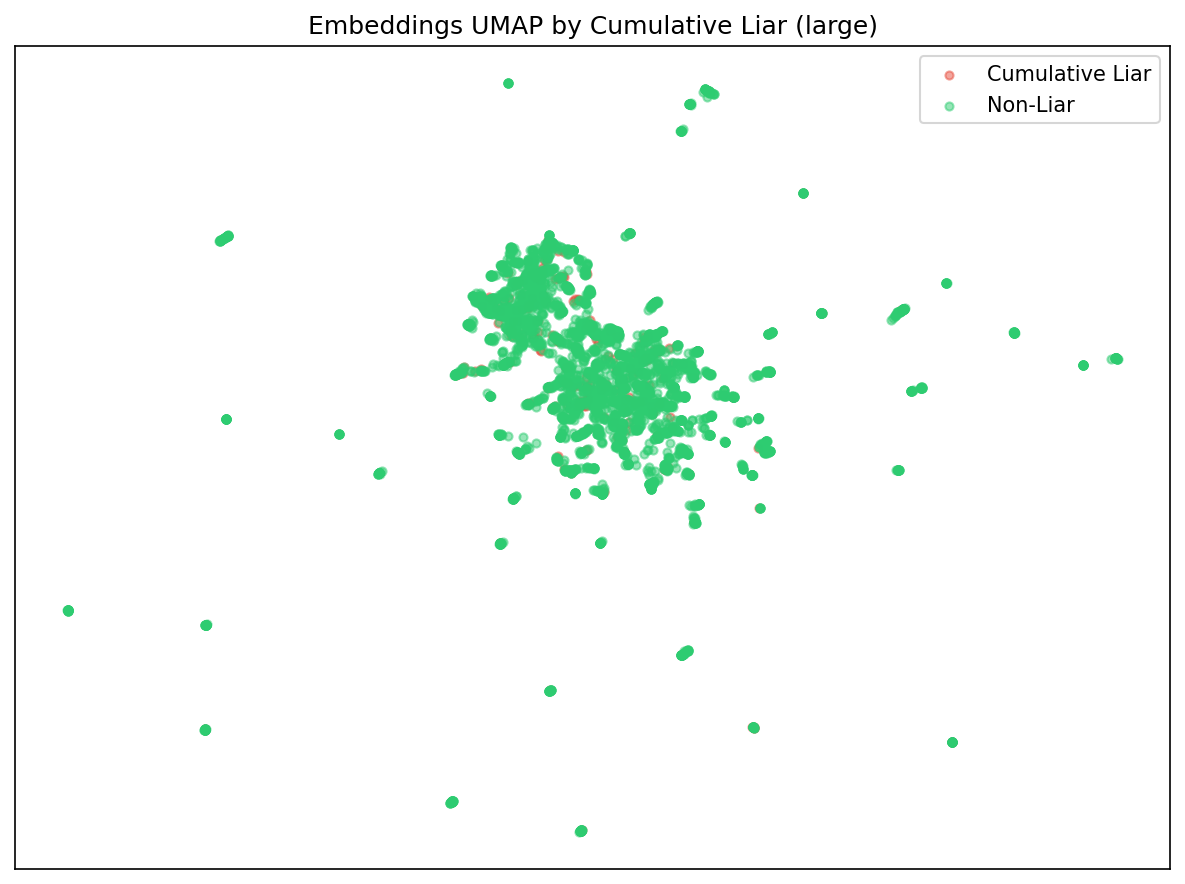
\includegraphics[width=\textwidth]{cumulative_liar_umap_large}
    \caption{UMAP --- cumulative liar}
\end{subfigure}
\hfill
\begin{subfigure}[b]{0.48\textwidth}
    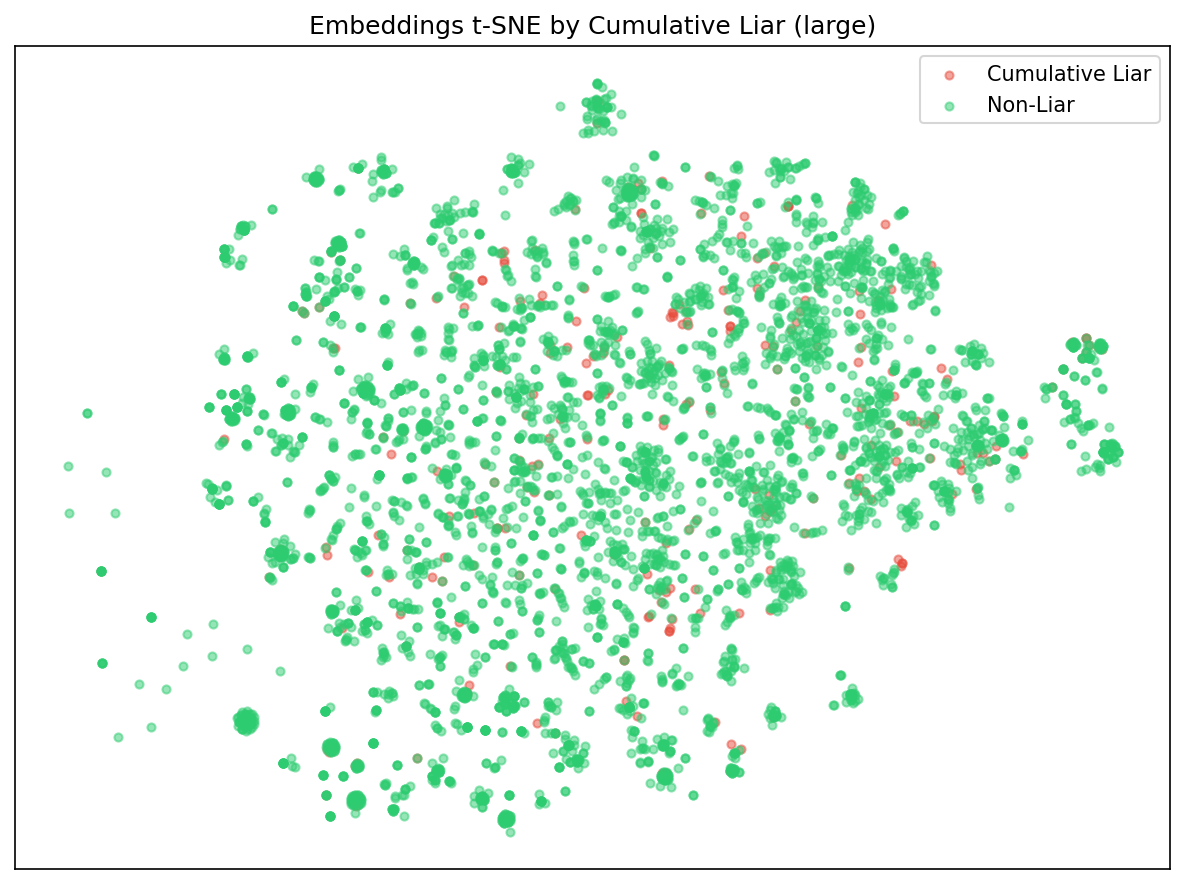
\includegraphics[width=\textwidth]{cumulative_liar_tsne_large}
    \caption{t-SNE --- cumulative liar}
\end{subfigure}
\caption{Message embeddings colored by cumulative-liar status (large model).}
\label{fig:cliar_dimreduce}
\end{figure}

\begin{figure}[H]
\centering
\begin{subfigure}[b]{0.48\textwidth}
    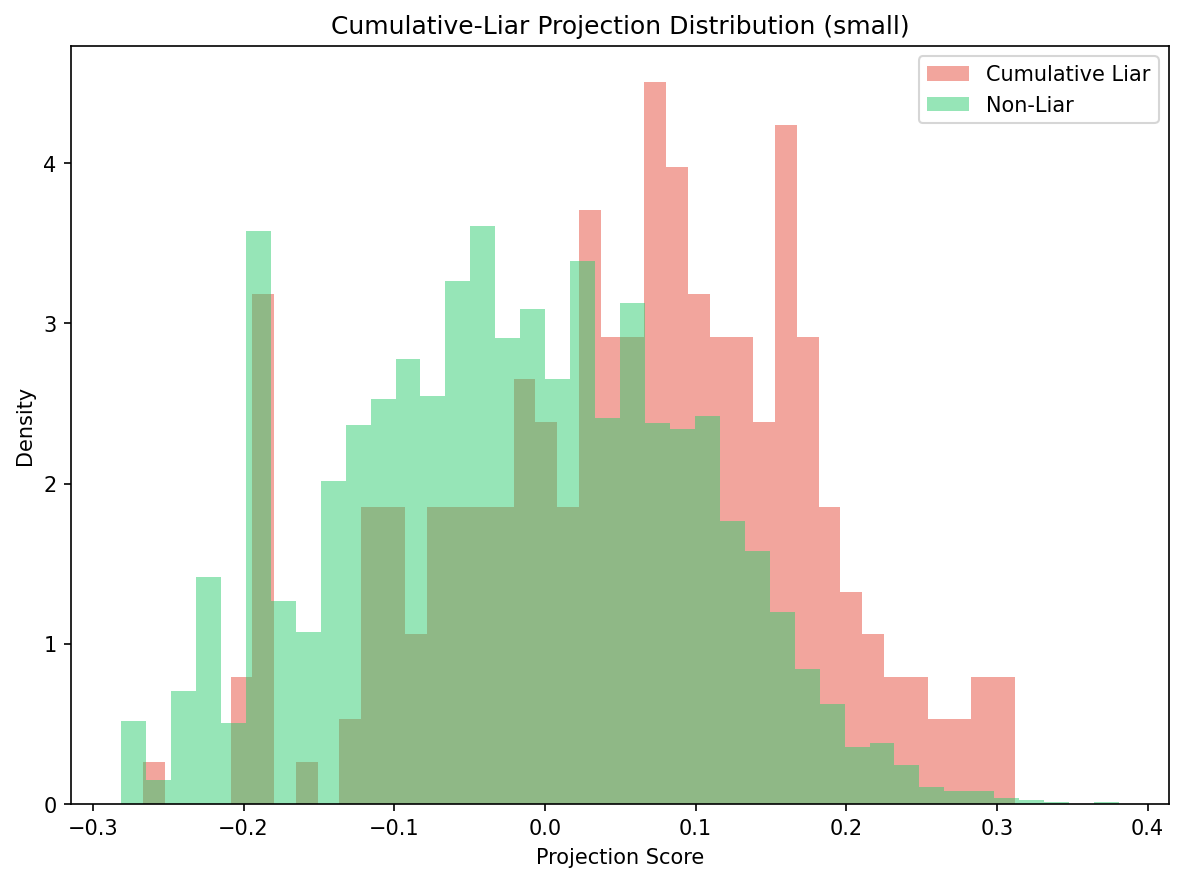
\includegraphics[width=\textwidth]{cumulative_liar_projection_dist_small}
    \caption{Small model}
\end{subfigure}
\hfill
\begin{subfigure}[b]{0.48\textwidth}
    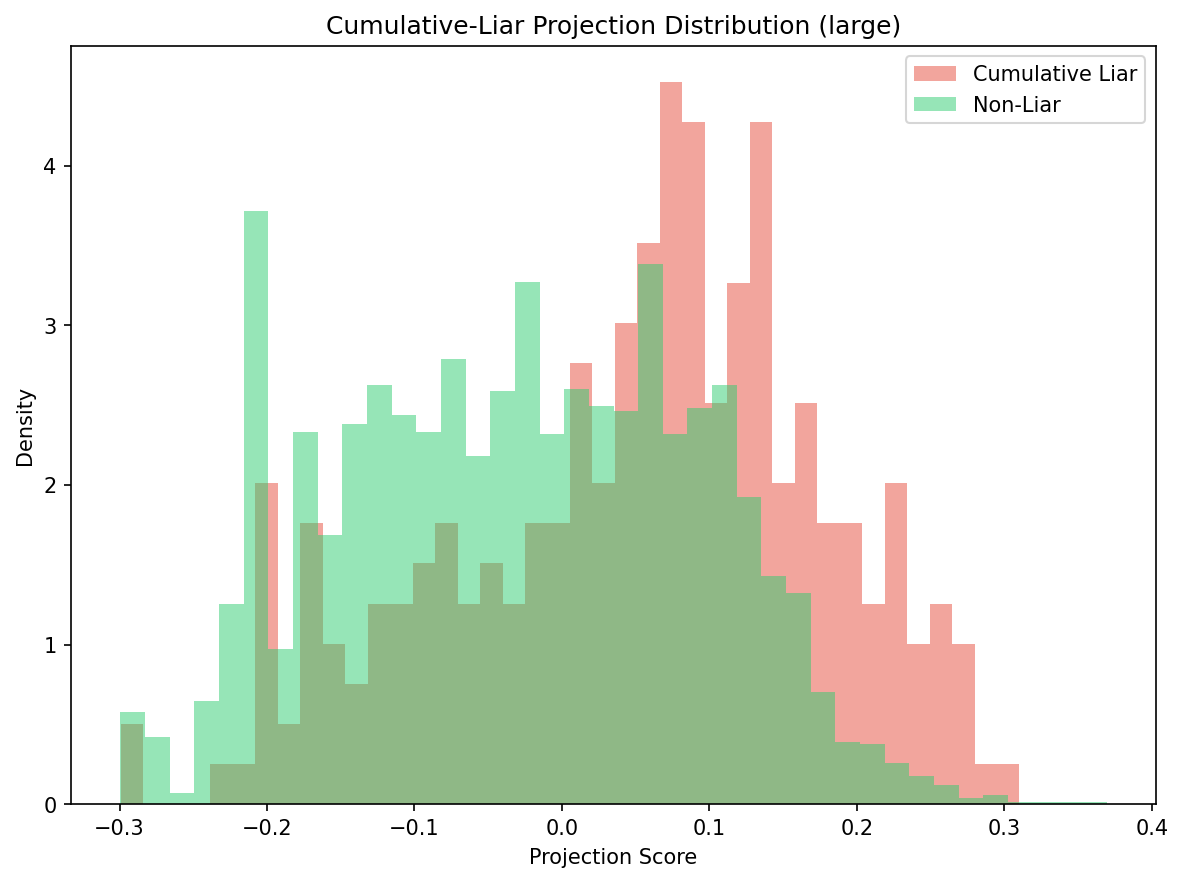
\includegraphics[width=\textwidth]{cumulative_liar_projection_dist_large}
    \caption{Large model}
\end{subfigure}
\caption{Cumulative-liar direction projection score distributions by state.}
\label{fig:cliar_projdist}
\end{figure}

\subsection{Projection Columns in Panel Dataset}

\begin{center}
\footnotesize
\begin{tabular}{ll}
\toprule
Column & Description \\
\midrule
\texttt{proj\_msg\_dir\_\{small,large\}} & Cooperative direction, message-level \\
\texttt{proj\_pr\_dir\_\{small,large\}} & Cooperative direction, player-round \\
\texttt{proj\_promise\_msg\_dir\_\{small,large\}} & Promise direction, message-level \\
\texttt{proj\_promise\_pr\_dir\_\{small,large\}} & Promise direction, player-round \\
\texttt{proj\_homog\_msg\_dir\_\{small,large\}} & Homogeneity direction, message-level \\
\texttt{proj\_homog\_pr\_dir\_\{small,large\}} & Homogeneity direction, player-round \\
\texttt{proj\_rliar\_msg\_dir\_\{small,large\}} & Round-liar direction, message-level \\
\texttt{proj\_rliar\_pr\_dir\_\{small,large\}} & Round-liar direction, player-round \\
\texttt{proj\_cliar\_msg\_dir\_\{small,large\}} & Cumulative-liar direction, message-level \\
\texttt{proj\_cliar\_pr\_dir\_\{small,large\}} & Cumulative-liar direction, player-round \\
\bottomrule
\end{tabular}
\end{center}

All columns are aggregated to the player-round level (mean across messages) and are \texttt{NaN} for round 1.

\end{document}
